\section{\trTerminalObject{}与\trInitialObject{}}
\label{sec:terminal-initial-objects}

在本节中，我们将讨论\trTerminalObject{}与\trInitialObject{}，作为对后文
∞-\trCategories{}中的\trLimit{}与\trColimit{}概念的热身。我们将给出若干条标准的
等价刻画，分别判别一个\trObject{}何时是终的、何时是始的。

\begin{definition}\label{def:initial-terminal}
设 $\C$ 是一个∞-\trCategory{}。\trObject{} $x$ 称为\emph{始的}（initial），如果对
$\C$ 的一切\trObject{} $y$，\trMappingSpace{} $\mathrm{map}_{\C}(x, y)$ 是%
\trContractible{}。同样地，称 $x$ 为\emph{终的}（terminal），如果它在
$\C^{\mathrm{op}}$ 中是始的；也就是说，如果对一切其他\trObject{} $y$，
\trMappingSpace{} $\mathrm{map}_{\C}(y, x)$ 是\trContractible{}。
\end{definition}

下列这些刻画将会是有用的。

\begin{lemma}\label{lem:terminal-characterizations}
设 $\C$ 是一个∞-\trCategory{}，$x$ 是 $\C$ 的一个\trObject{}。那么，下列条件等价：
\begin{enumerate}[label=(\arabic*)]
  \item $x$ 是终的。
  \item \trFunctor{} $\C_{/x} \to \C$ 是一个\trTrivialFibration{}。
  \item 对每个 $n \ge 1$，每个\trLiftingProblem{}%
\begin{center}
\begin{tikzpicture}
  \node (v) at (0,0) {$\Delta^{\{n\}}$};
  \node (bd) at (2.6,0) {$\partial\Delta^n$};
  \node (c) at (5.2,0) {$\C$};
  \node (dn) at (2.6,-1.7) {$\Delta^n$};
  \draw[->] (v) -- (bd);
  \draw[->] (bd) -- (c);
  \draw[->] (bd) -- (dn);
  \draw[->, dashed] (dn) -- (c);
  \draw[->, bend left=25] (v) to node[above] {$x$} (c);
\end{tikzpicture}
\end{center}
容有一个解。
\end{enumerate}
\end{lemma}

\begin{proof}
为了证明（1）与（2）等价，我们考虑图表
\begin{center}
\begin{tikzpicture}
  \node (cx) at (0,0) {$\C_{/x}$};
  \node (c1) at (3.6,0) {$\C$};
  \node (c2) at (2.0,-1.8) {$\C$};
  \draw[->] (cx) -- (c1);
  \draw[->] (cx) -- (c2);
  \draw[double, double distance=1.2pt] (c1) -- (c2);
\end{tikzpicture}
\end{center}
并希望证明水平映射是一个\trTrivialFibration{}。我们已经知道它是一个%
\trRightFibration{}，故只需证明：它是一个\trJoyalEquivalence{}当且仅当 $x$ 是终的。
由第 3 章中的\cref{thm:fibrewise-criterion}，该映射是一个\trJoyalEquivalence{}%
当且仅当它逐纤维地是\trJoyalEquivalence{}，而这相当于说：对 $\C$ 的一切\trObject{}%
$y$，典范映射 $\mathrm{map}^R_{\C}(y, x) \to \Delta^0$ 是一个\trJoyalEquivalence{}。

为了看出（2）与（3）等价，我们观察到，映射
\[
\partial\Delta^{n-1} \star \Delta^0
  \amalg_{\partial\Delta^{n-1} \star \varnothing}
  \Delta^{n-1} \star \varnothing
  \longrightarrow \Delta^{n-1} \star \Delta^0
\]
同构于映射
\[
\partial\Delta^n \longrightarrow \Delta^n.
\]
于是，\trLiftingProblem{}%
\begin{center}
\begin{tikzpicture}
  \node (v) at (0,0) {$\Delta^{\{n\}}$};
  \node (bd) at (2.6,0) {$\partial\Delta^n$};
  \node (c) at (5.2,0) {$\C$};
  \node (dn) at (2.6,-1.7) {$\Delta^n$};
  \draw[->] (v) -- (bd);
  \draw[->] (bd) -- (c);
  \draw[->] (bd) -- (dn);
  \draw[->, dashed] (dn) -- (c);
  \draw[->, bend left=25] (v) to node[above] {$x$} (c);
\end{tikzpicture}
\end{center}
等价于\trLiftingProblem{}%
\begin{center}
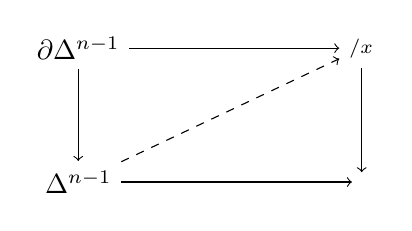
\begin{tikzpicture}
  \node (bd) at (0,0) {$\partial\Delta^{n-1}$};
  \node (cx) at (3.6,0) {$\C_{/x}$};
  \node (dn) at (0,-1.7) {$\Delta^{n-1}$};
  \node (c) at (3.6,-1.7) {$\C$};
  \draw[->] (bd) -- (cx);
  \draw[->] (bd) -- (dn);
  \draw[->] (cx) -- (c);
  \draw[->] (dn) -- (c);
  \draw[->, dashed] (dn) -- (cx);
\end{tikzpicture}
\end{center}
因此，本引理得证。
\end{proof}

下面的结果告诉我们，\trInitialObject{}与\trTerminalObject{}若存在，则它们在%
\trContractible{}选择下是唯一的。

\begin{proposition}\label{prop:terminal-contractible}
设 $\C$ 是一个∞-\trCategory{}，并设 $\C_{\mathrm{term}}$ 为由 $\C$ 的全部%
\trTerminalObject{}组成的满子范畴。那么，$\C_{\mathrm{term}}$ 要么为空，要么是一个%
\trContractible{}\trKanComplex{}。
\end{proposition}

\begin{proof}
设 $\C_{\mathrm{term}}$ 非空。我们需要证明：任何\trLiftingProblem{}%
\begin{center}
\begin{tikzpicture}
  \node (bd) at (0,0) {$\partial\Delta^n$};
  \node (ct) at (3,0) {$\C_{\mathrm{term}}$};
  \node (dn) at (0,-1.5) {$\Delta^n$};
  \draw[->] (bd) -- (ct);
  \draw[->] (bd) -- (dn);
  \draw[->, dashed] (dn) -- (ct);
\end{tikzpicture}
\end{center}
容有一个解。若 $n = 0$，则由 $\C_{\mathrm{term}}$ 非空这一假设，解存在。若 $n \ge 1$，
我们使用\cref{lem:terminal-characterizations}的（3），这是可能的，因为特别地，
$\partial\Delta^n$ 的\trObject{} $\Delta^{\{n\}}$ 被送到一个\trTerminalObject{}。
\end{proof}

\begin{lemma}\label{lem:initial-left-anodyne}
设 $\C$ 是一个∞-\trCategory{}。那么，$\C$ 的一个\trObject{} $x$ 是始的，当且仅当映射
$x\colon \Delta^0 \to \C$ 是\trLeftAnodyne{}的。对偶地，若映射 $\Delta^0 \to \C$
是\trRightAnodyne{}的，则 $x$ 是终的。
\end{lemma}

\begin{proof}
我们对\trInitialObject{}证明本引理；\trTerminalObject{}的情形由过渡到\trOppositeCategory{}得到。
我们首先观察到：对任何%
\trMonomorphism{} $S \to T$，映射 $S \star \Delta^0 \to T \star \Delta^0$ 是%
\trRightAnodyne{}的，而映射 $\Delta^0 \star S \to \Delta^0 \star T$ 是%
\trLeftAnodyne{}的：为看出这一点，只需处理 $S \to T$ 为\trBoundaryInclusion{}%
$\partial\Delta^n \to \Delta^n$ 的情形，此时所论映射成为
$\Lambda^{n+1}_{n+1} \to \Delta^{n+1}$ 与 $\Lambda^{n+1}_0 \to \Delta^{n+1}$。
现在设 $x$ 是始的。由\cref{lem:terminal-characterizations}的\trInitialObject{}版本，
我们发现
$\C_{x/} \to \C$ 是一个\trTrivialFibration{}。我们选取一个\trSectionMap{}%
$s\colon \C \to \C_{x/}$，并考虑图表
\begin{center}
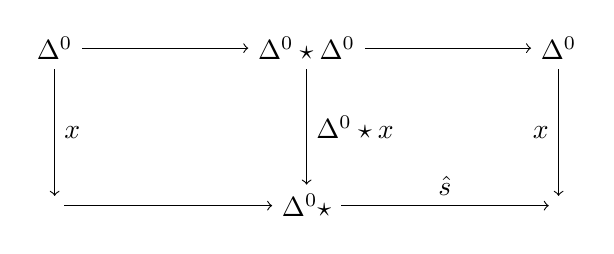
\begin{tikzpicture}
  \node (d0a) at (0,0) {$\Delta^0$};
  \node (st) at (3.2,0) {$\Delta^0 \star \Delta^0$};
  \node (d0b) at (6.4,0) {$\Delta^0$};
  \node (ca) at (0,-2.0) {$\C$};
  \node (cs) at (3.2,-2.0) {$\Delta^0 \star \C$};
  \node (cb) at (6.4,-2.0) {$\C$};
  \draw[->] (d0a) -- (st);
  \draw[->] (st) -- (d0b);
  \draw[->] (ca) -- (cs);
  \draw[->] (cs) -- node[above] {$\hat{s}$} (cb);
  \draw[->] (d0a) -- node[right] {$x$} (ca);
  \draw[->] (st) -- node[right] {$\Delta^0 \star x$} (cs);
  \draw[->] (d0b) -- node[left] {$x$} (cb);
\end{tikzpicture}
\end{center}
其中 $\hat{s}$ 是 $s$ 的\trAdjunction{}映射。由此可知，两个水平复合都是恒等。因此，映射
$\Delta^0 \xrightarrow{x} \C$ 是映射 $\Delta^0 \star x$ 的一个\trRetract{}，而由我们
先前的观察，后者是\trLeftAnodyne{}的。

反之，假设 $\Delta^0 \xrightarrow{x} \C$ 是\trLeftAnodyne{}的。我们可以考虑图表
\begin{center}
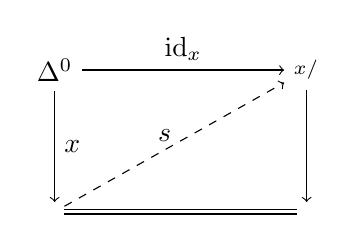
\begin{tikzpicture}
  \node (d0) at (0,0) {$\Delta^0$};
  \node (cx) at (3.2,0) {$\C_{x/}$};
  \node (c1) at (0,-1.8) {$\C$};
  \node (c2) at (3.2,-1.8) {$\C$};
  \draw[->] (d0) -- node[above] {$\mathrm{id}_x$} (cx);
  \draw[->] (d0) -- node[right] {$x$} (c1);
  \draw[->] (cx) -- (c2);
  \draw[double, double distance=1.2pt] (c1) -- (c2);
  \draw[->, dashed] (c1) -- node[pos=0.5, above left, inner sep=1pt] {$s$} (cx);
\end{tikzpicture}
\end{center}
并找到一条使图表交换的虚箭头 $s$。我们将通过建立\cref{lem:terminal-characterizations}
的（3）来证明 $x$ 是始的。于是，我们考虑图表
\begin{center}
\begin{tikzpicture}
  \node (v) at (0,0) {$\Delta^{\{0\}}$};
  \node (bd) at (2.6,0) {$\partial\Delta^n$};
  \node (c1) at (5.2,0) {$\C$};
  \node (cx) at (7.4,0) {$\C_{x/}$};
  \node (c2) at (10,0) {$\C$};
  \node (dn) at (2.6,-1.8) {$\Delta^n$};
  \draw[->] (v) -- (bd);
  \draw[->] (bd) -- (c1);
  \draw[->] (c1) -- node[above] {$s$} (cx);
  \draw[->] (cx) -- (c2);
  \draw[->] (bd) -- (dn);
  \draw[->, dashed] (dn) -- (c1);
  \draw[->, dotted] (dn) -- (cx);
  \draw[->, bend left=25] (v) to node[above] {$x$} (c1);
\end{tikzpicture}
\end{center}
由构造，我们有 $s(x) = \mathrm{id}_x$，于是由\cref{ex:terminal-object-slice}，它是 $\C_{x/}$ 的一个%
\trInitialObject{}。故点箭头存在，从而虚箭头也存在。
\end{proof}

\begin{proposition}\label{prop:initial-terminal-in-fun}
设 $\C$ 是一个∞-\trCategory{}，并设 $K$ 是一个\trSimplicialSet{}。设给定一个%
\trFunctor{} $F\colon K \to \C$，使得对 $K$ 的一切\trObject{} $x$，\trObject{}%
$F(x)$ 在 $\C$ 中是始的（相应地，终的）。那么，$F$ 在 $\mathrm{Fun}(K, \C)$ 中是
始的（相应地，终的）。
\end{proposition}

\begin{proof}
我们证明\trTerminalObject{}的情形。我们需要证明：对一切 $n \ge 1$，任何\trLiftingProblem{}%
\begin{center}
\begin{tikzpicture}
  \node (v) at (0,0) {$\Delta^{\{n\}}$};
  \node (bd) at (2.6,0) {$\partial\Delta^n$};
  \node (f) at (5.8,0) {$\mathrm{Fun}(K, \C)$};
  \node (dn) at (2.6,-1.8) {$\Delta^n$};
  \draw[->] (v) -- (bd);
  \draw[->] (bd) -- node[above] {$\hat{F}$} (f);
  \draw[->] (bd) -- (dn);
  \draw[->, dashed] (dn) -- (f);
  \draw[->, bend left=25] (v) to node[above] {$F$} (f);
\end{tikzpicture}
\end{center}
容有一个解。经\trAdjunction{}，这对应于\trLiftingProblem{}%
\begin{center}
\begin{tikzpicture}
  \node (v) at (0,0) {$K \times \Delta^{\{n\}}$};
  \node (bd) at (3.6,0) {$K \times \partial\Delta^n$};
  \node (c) at (6.3,0) {$\C$};
  \node (dn) at (3.6,-1.8) {$K \times \Delta^n$};
  \draw[->] (v) -- (bd);
  \draw[->] (bd) -- (c);
  \draw[->] (bd) -- (dn);
  \draw[->, dashed] (dn) -- (c);
  \draw[->, bend left=25] (v) to node[above] {$F$} (c);
\end{tikzpicture}
\end{center}
其中，由假设，上方水平复合沿任何\trObject{} $x\colon \Delta^0 \to K$ 的进一步限制都是
$\C$ 的一个\trTerminalObject{}。我们考虑\trFiltration{}%
$F_k(K) = \mathrm{sk}_k(K \times \Delta^n) \cup K \times \partial\Delta^n$，
并希望归纳地求解下述\trExtensionProblem{}：
\begin{center}
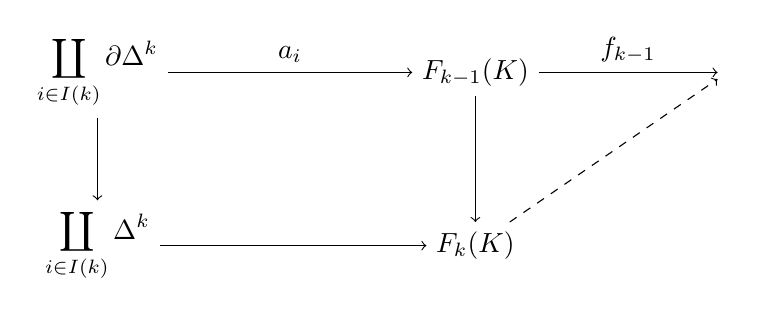
\begin{tikzpicture}
  \node (bd) at (0,0) {$\displaystyle\coprod_{i \in I(k)} \partial\Delta^k$};
  \node (f1) at (4.8,0) {$F_{k-1}(K)$};
  \node (c) at (8,0) {$\C$};
  \node (dn) at (0,-2.2) {$\displaystyle\coprod_{i \in I(k)} \Delta^k$};
  \node (fk) at (4.8,-2.2) {$F_k(K)$};
  \draw[->] (bd) -- node[above] {$a_i$} (f1);
  \draw[->] (f1) -- node[above] {$f_{k-1}$} (c);
  \draw[->] (bd) -- (dn);
  \draw[->] (dn) -- (fk);
  \draw[->] (f1) -- (fk);
  \draw[->, dashed] (fk) -- (c);
\end{tikzpicture}
\end{center}
为此，只需观察到：对一切 $i \in I(k)$，复合 $f_{k-1} \circ a_i$ 把顶点 $\{k\}$ 送到
$\C$ 中的一个\trTerminalObject{}。由定义，$I(k)$ 由 $K \times \Delta^n$ 的那些
不含于 $K \times \partial\Delta^n$ 的非退化 $k$-\trSimplex{}组成；换言之，$I(k)$ 的
成员特别地是形如 $(\alpha_i, \beta_i) \in K_k \times \Delta^n_k$ 的对，其中
$\beta_i\colon [k] \to [n]$ 是满射。\footnote{译注：原书此处印作
「$b\colon [k] \to [n]$ 是满射」，按上下文应为 $\beta_i$，此处径改。——译者注}
特别地，$\beta_i$ 把\trObject{} $\{k\}$ 送到 $\{n\}$。于是
$f_{k-1}(a_i(\{k\})) = \hat{F}(\alpha_i(\{k\}, \{n\}))$，由假设，它是一个%
\trTerminalObject{}。故虚箭头存在。对 $k$ 过渡到\trColimit{}，本命题即得证。
\end{proof}

\cref{prop:initial-terminal-in-fun}的逆命题几乎成立，正如下面的引理所揭示的。

\begin{lemma}\label{lem:terminal-values}
设 $\C_{\mathrm{term}}$ 非空。那么，$\mathrm{Fun}(K, \C)$ 的任何\trTerminalObject{}%
都取值于 $\C_{\mathrm{term}}$ 中。
\end{lemma}

\begin{proof}
设 $x$ 是一个\trTerminalObject{}，并考虑取值为 $x$ 的\trConstantFunctor{} $c_x$。由%
\cref{prop:initial-terminal-in-fun}，$c_x$ 是 $\mathrm{Fun}(K, \C)$ 的一个%
\trTerminalObject{}。由\cref{prop:terminal-contractible}，$\mathrm{Fun}(K, \C)$ 的
任何其他\trTerminalObject{} $T$ 都等价于 $c_x$。特别地，对 $K$ 的任何\trObject{}%
$k$，我们有：$T(k)$ 等价于 $c_x(k)$，从而它是终的。
\end{proof}
